\subsection{Unsicherheitsrechnung}\label{VGuD}

%TODO Unsicherheiten?

\subsection{Oszilloskopkurven}

%	\begin{figure}[ht]
%		\centering
%		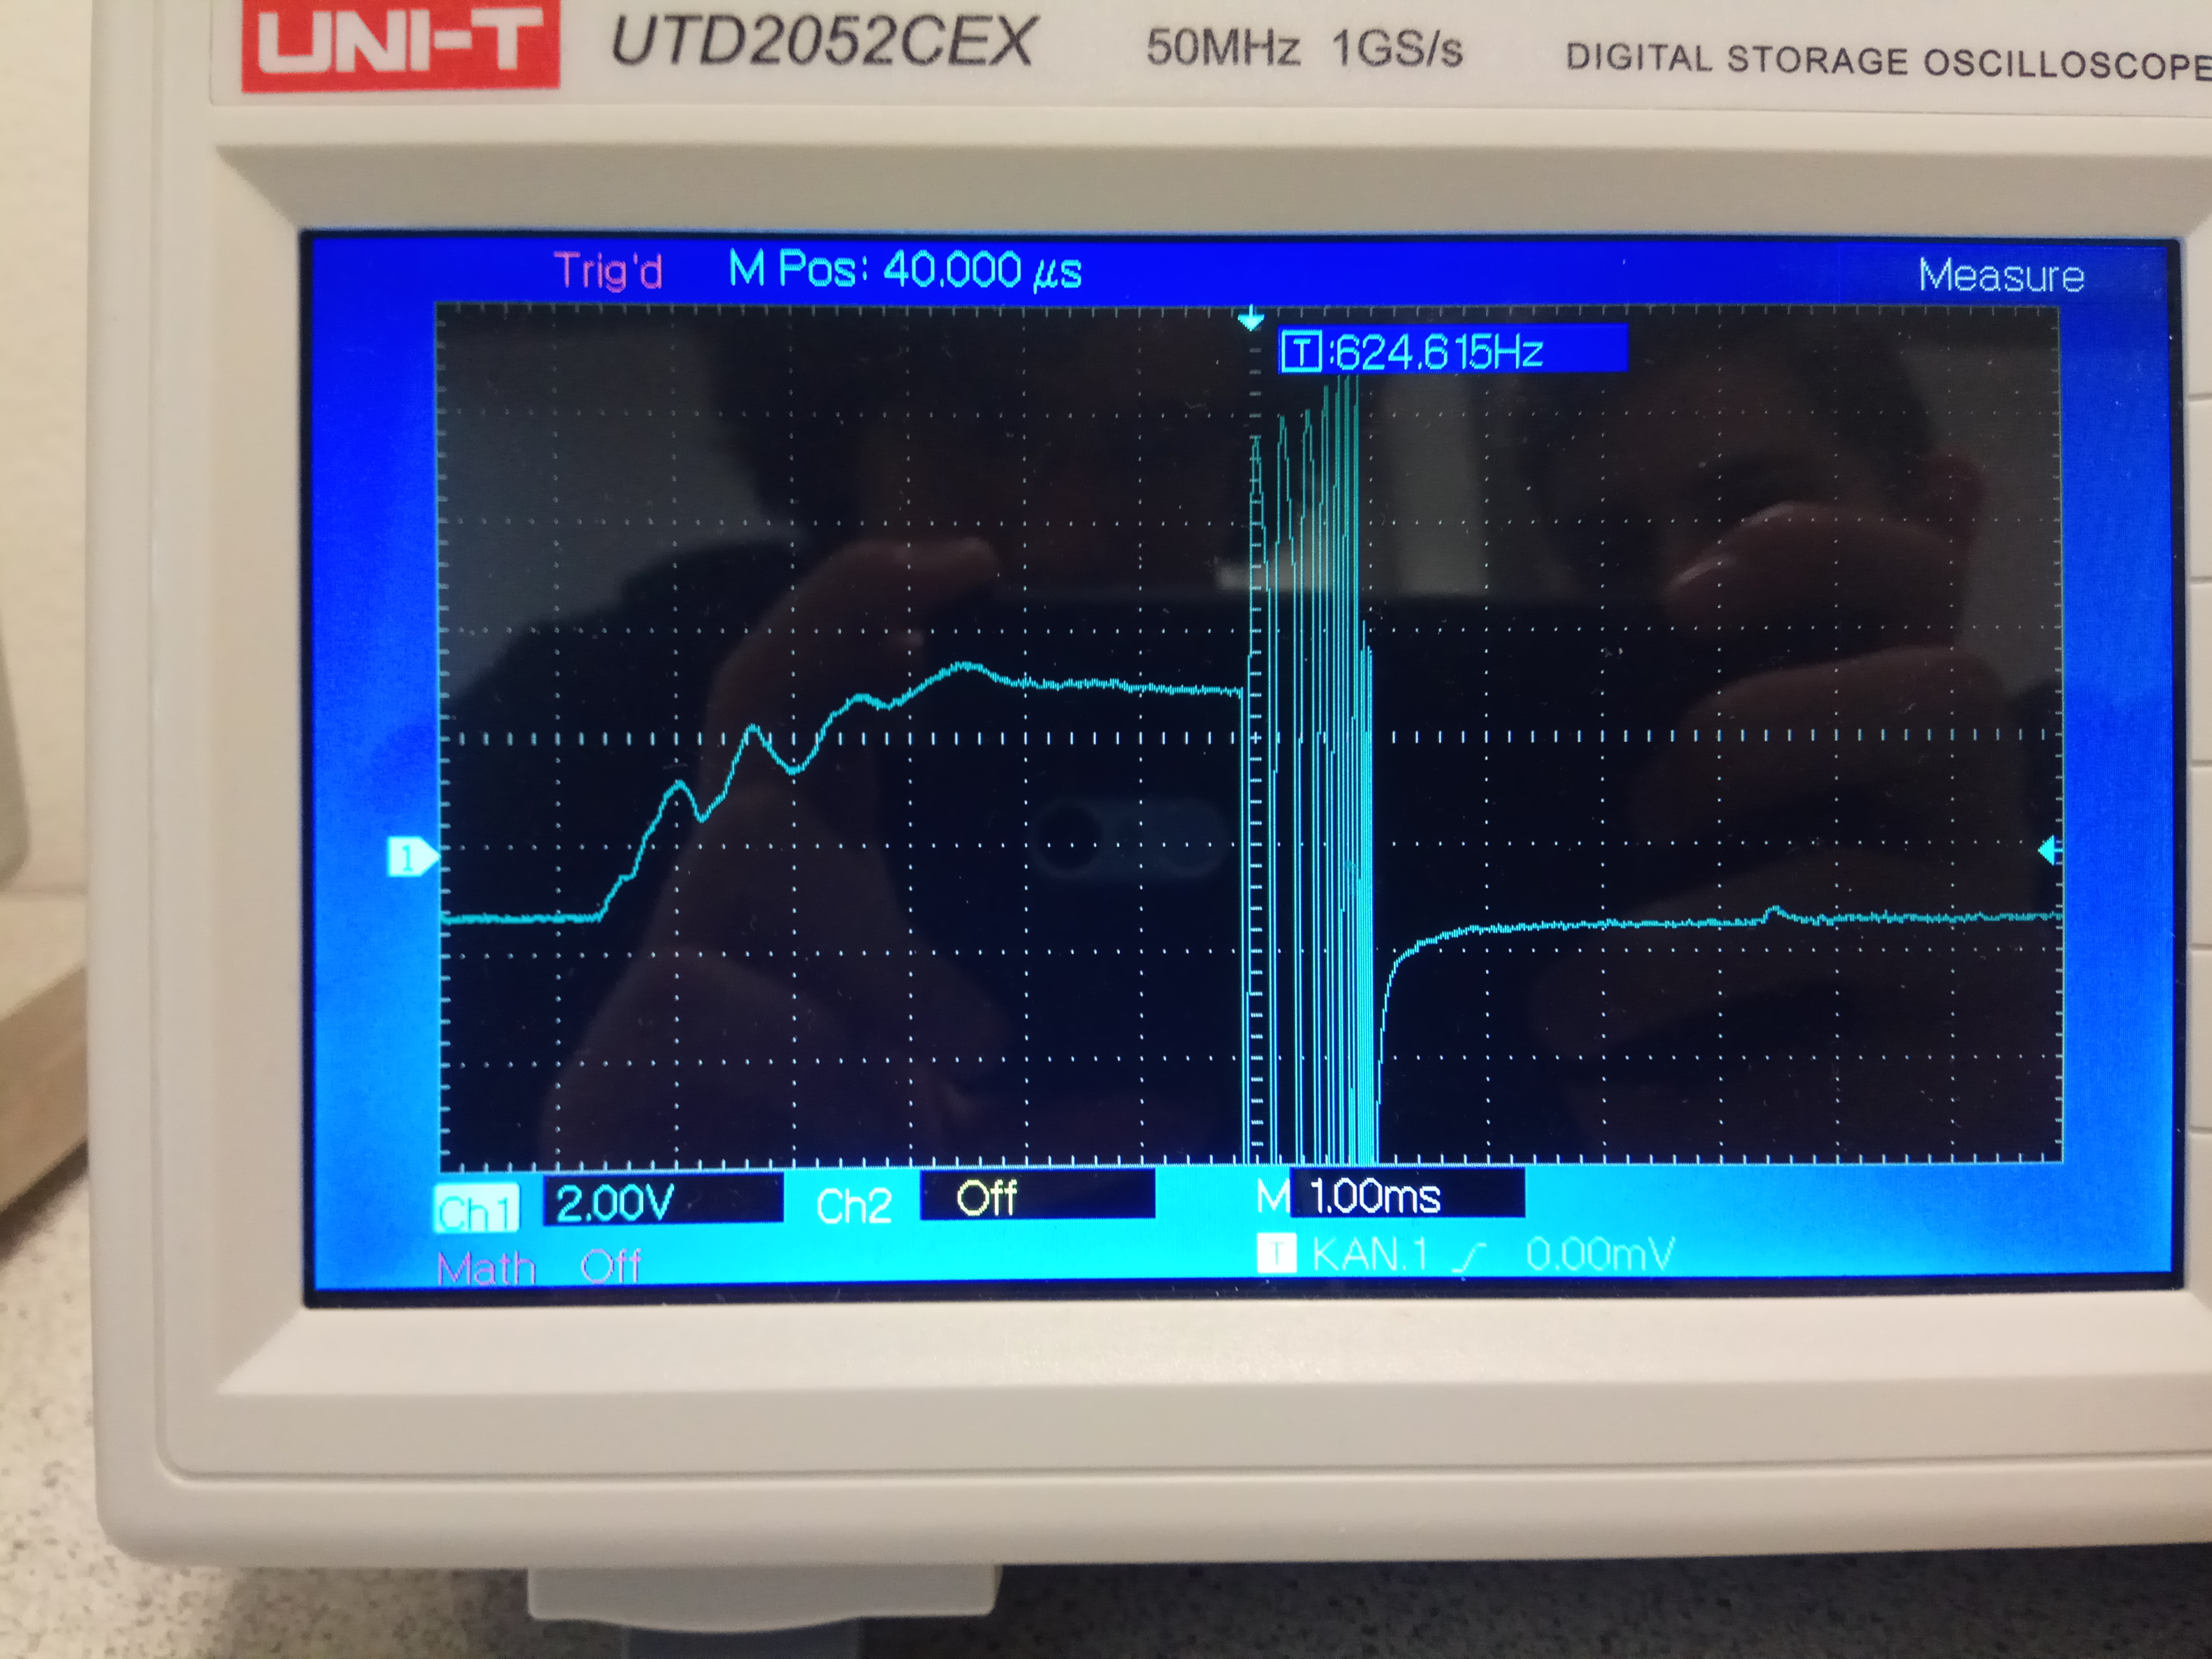
\includegraphics[width=\textwidth]{bilder/ne.jpg}
%		\caption{Franck-Hertz-Kurve des Neons am Oszilloskop.
%		\label{fig:kurveNe}	
%	\end{figure}

%	\begin{figure}[ht]
%		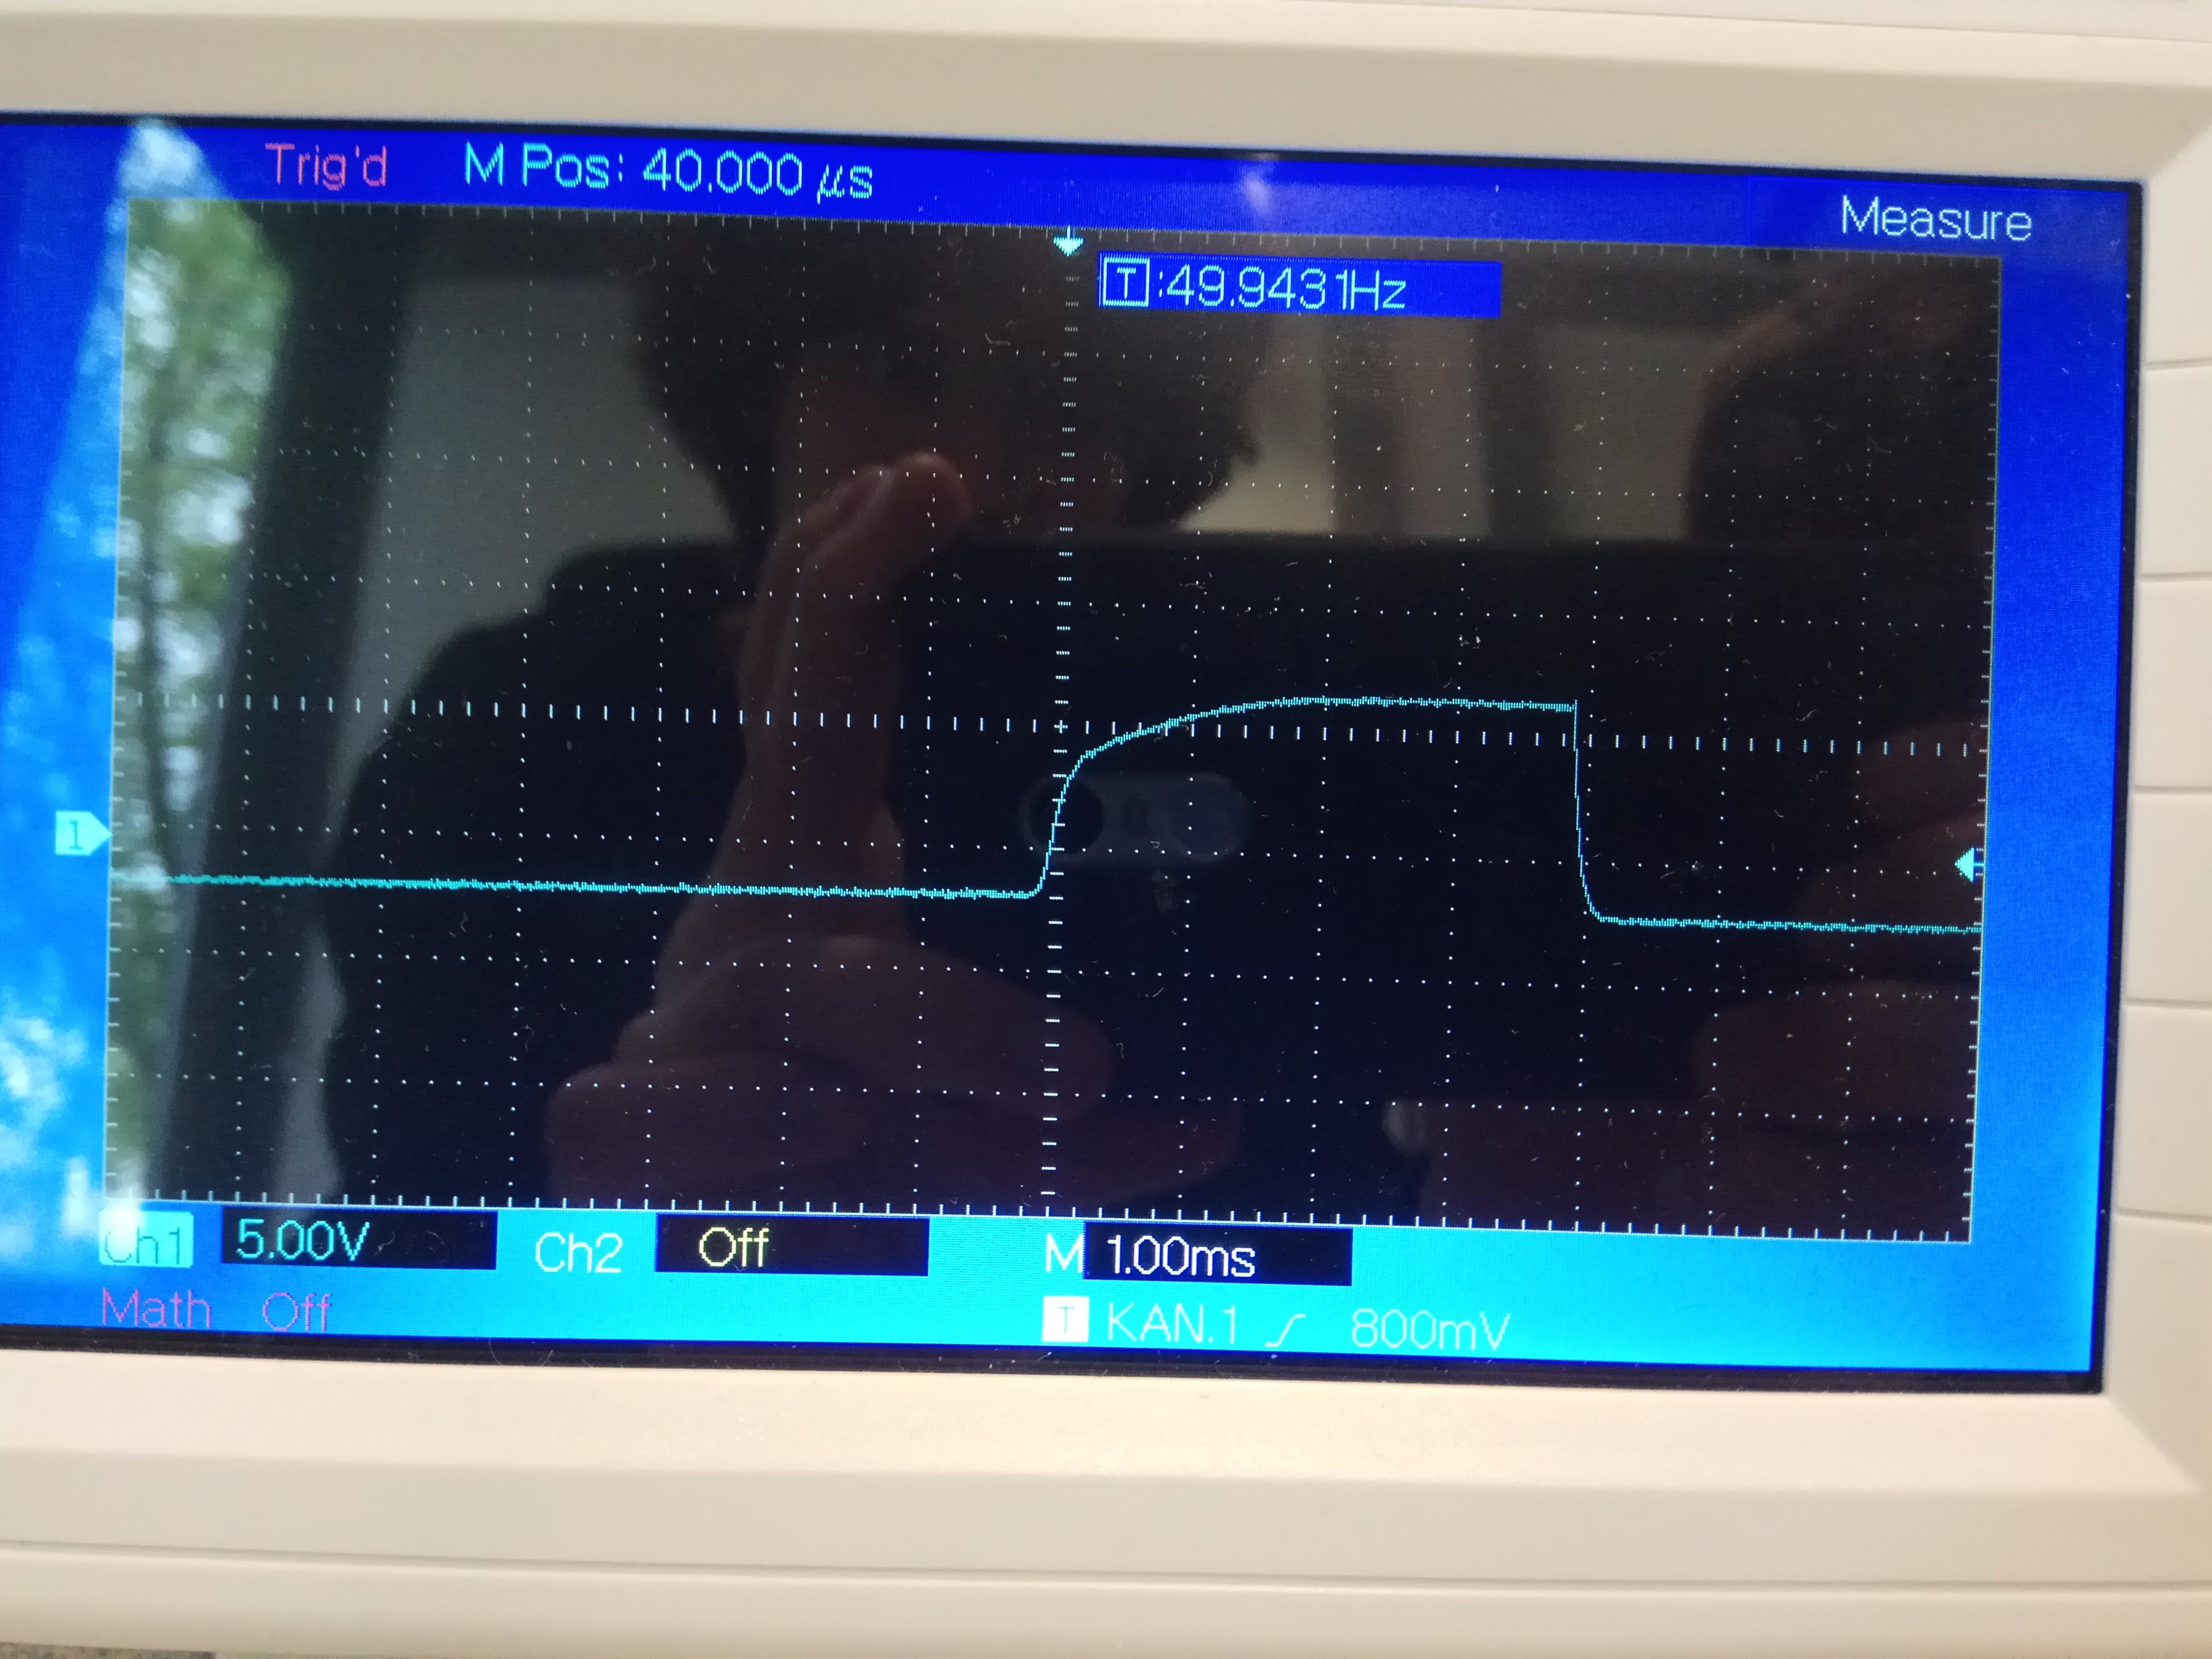
\includegraphics[width=\textwidth]{bilder/hgl.jpg}
%		\caption{Franck-Hertz-Kurve des Quecksilbers bei Raumtemperatur am Oszilloskop.}
%		\label{fig:kurveHgl}	
%	\end{figure}
	
%	\begin{figure}[ht]
%		\centering
%		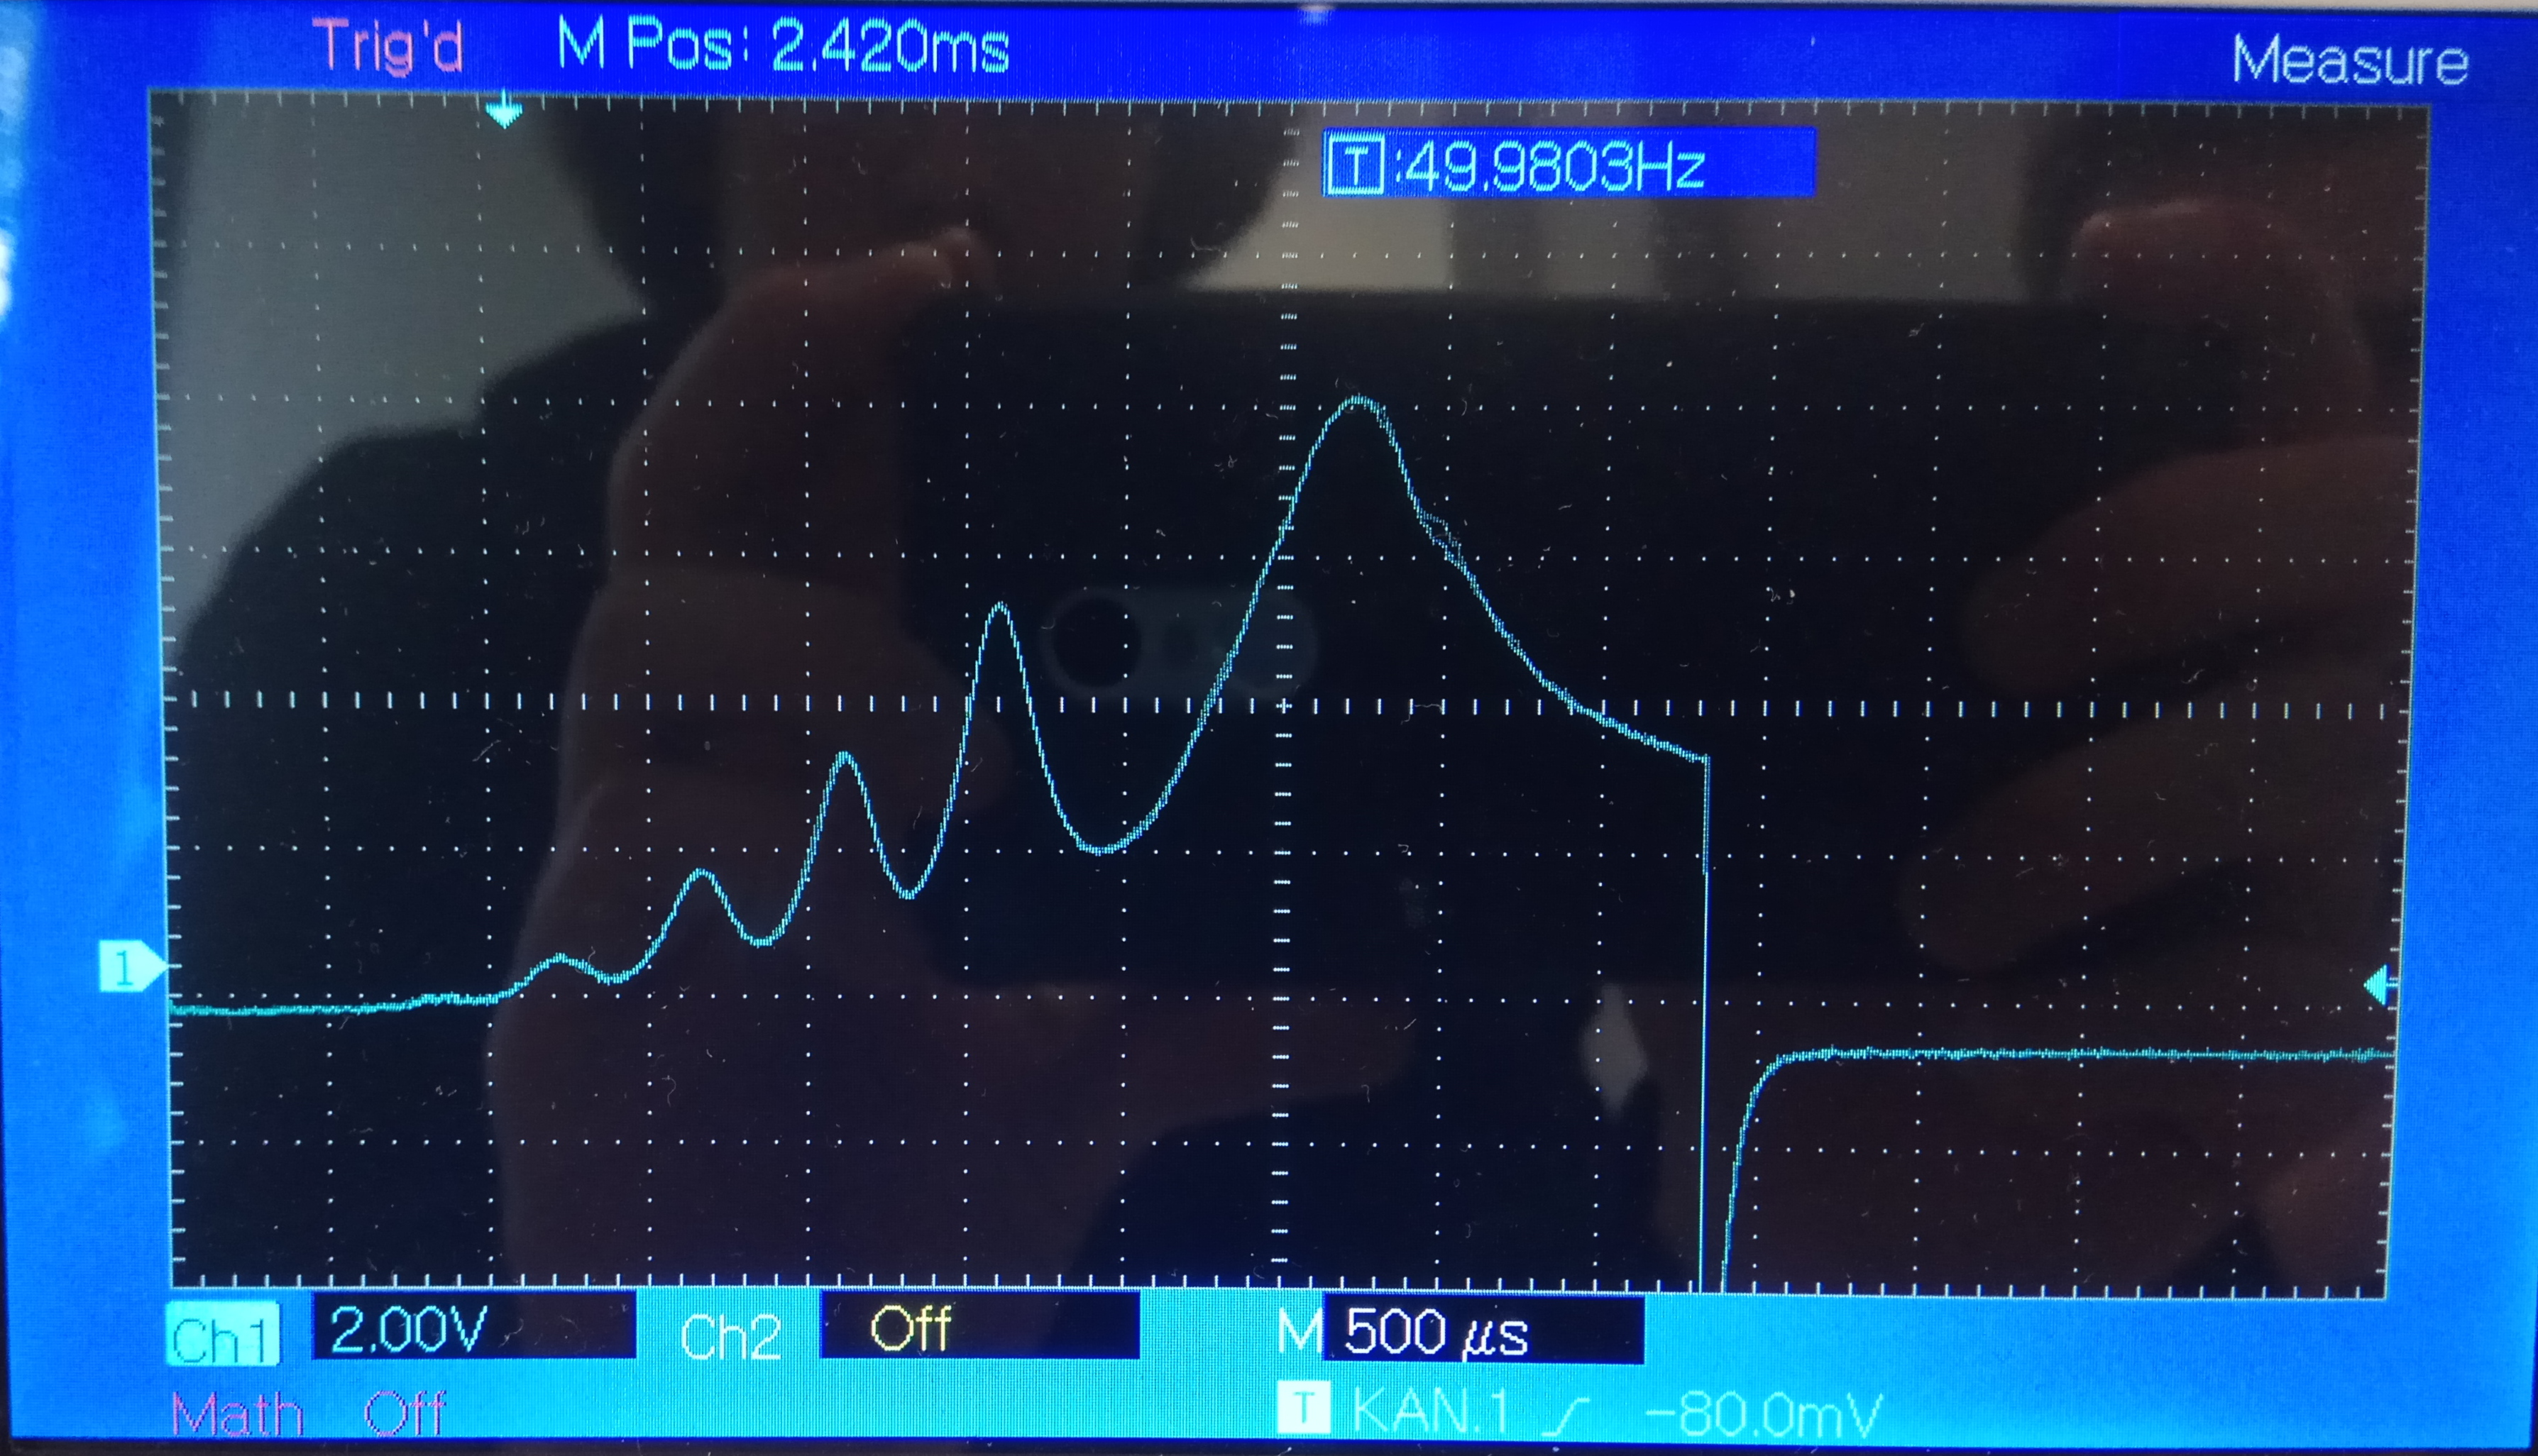
\includegraphics[width=\textwidth]{bilder/hgg.jpg}
%		\caption{Franck-Hertz-Kurve des erhitzten Quecksilbers am Oszilloskop.}
%		\label{fig:kurveHgg}	
%	\end{figure}	
